\documentclass{article}
\usepackage[utf8]{inputenc}

\title{Project 2}
\author{Ahren Roth, Yifeng Qin }
\date{CS 491/691 October 2019}

\usepackage{natbib}
\usepackage{graphicx}

\begin{document}

\maketitle

\section{KNN\_test(X\_train,Y\_train,X\_test,Y\_test,K)}
This function uses a set of training features and corresponding labels to make predictions on a set of test features and their corresponding labels. For each point in the test set, Euclidean distances are calculated to each of the points in the training set. The majority vote between the labels of the K minimum distances, where K is an odd integer less than the count of training points, determines the value of the prediction for the test point. This process is repeated for each point in the test set. Each prediction is compared with the corresponding label value of the test set and an accuracy score on the entire set is returned.

\section{KNN Classifications On Test Data}
\begin{tabular}{c | c | c | c}
\hline
     Test & K = 1 & K = 3 & K = 5 \\ \hline
     1 & -1 & -1 & 1\\
     2 & 1 & 1 & -1\\
     3 & 1 & 1 & -1\\
     4 & -1 & -1 & 1\\
     5 & -1 & -1 & -1\\
     6 & 1 & -1 & -1\\
     7 & 1 & 1 & 1\\
     8 & 1 & 1 & 1\\
     9 & -1 & -1 & 1\\
     10 & 1 & 1 & -1

\end{tabular}

\section{choose\_K(X\_train,Y\_train,X\_val,Y\_val)}
This function utilizes the KNN\_test function to classify each point in the test set and return an accuracy score for all odd values of K from 1 to the number of points in the training set. The K value with the highest accuracy score is returned.

\section{Best K Value For the Test Data}
K = 9 returns the highest accuracy on the training data. It is interesting to note that local minima are encountered while maximizing the accuracy.

\section{K\_Means(X,K)}
Takes as input training set X and the number of clusters K. Cluster centers are randomly generated by function Rand\_Cluster\_Centers(X,K). Cluster center features reside within the maximum and minimum values for each feature in the training set. Duplicate cluster centers are not allowed. For each cluster center a distance to each point in the training set is calculated using Find\_Distances(X, CC). In Build\_Clusters(X, K, AD) each point is 'clustered' around the cluster center that it is closest to. The cluster centers are recalculated in Calculate\_Cluster\_Centers(Clusters, Cluster\_Centers, XShape1) by averaging the values of each feature. This process is repeated until the cluster centers remain in the same position because the points in the training set remain with the cluster they are assigned. 

\section{K\_Means Cluster Plots}
The cluster centers indicated in the figures occur most frequently, but are not the only possible cluster centers returned by the K\_Means function.
\begin{figure}[h!]
\centering
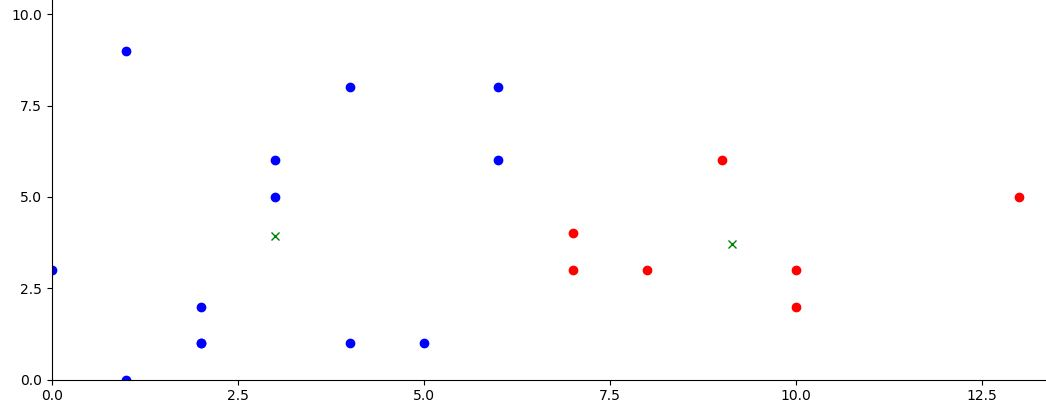
\includegraphics[scale=.5]{cluster_k2}
\caption{K = 2\newline Cluster Centers: \newline[9.142857142857142, 3.7142857142857144]\newline[3.0, 3.923076923076923]}
\label{fig:universe}
\end{figure}

\begin{figure}[h!]
\centering
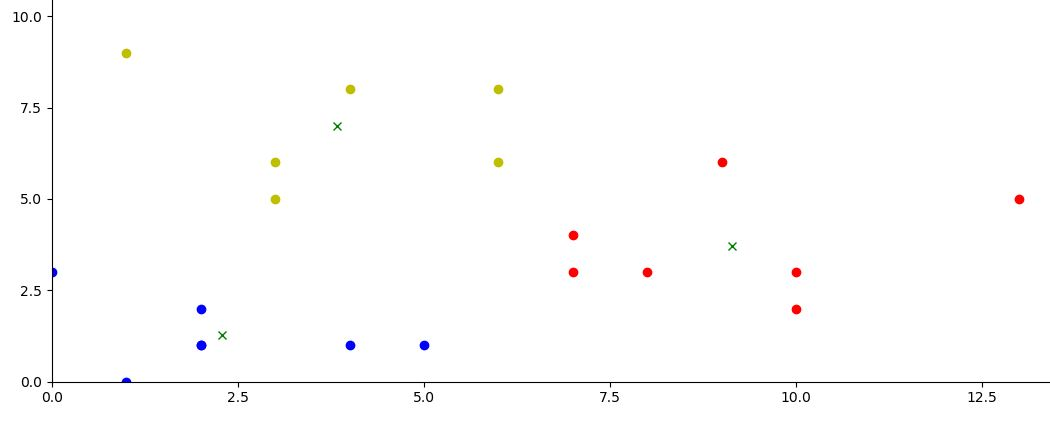
\includegraphics[scale=.5]{cluster_k3}
\caption{K = 3\newline Cluster Centers: \newline[9.142857142857142, 3.7142857142857144]\newline[2.2857142857142856, 1.2857142857142858]\newline[3.8333333333333335, 7.0]}
\label{fig:universe}
\end{figure}

\section{K\_Means\_better(X,K)}
This function runs 1000 iterations of K\_Means with a particular K value and returns the cluster centers that occur most frequently.

\section{K\_Means\_better Cluster Plots}


\begin{figure}[h!]
\centering
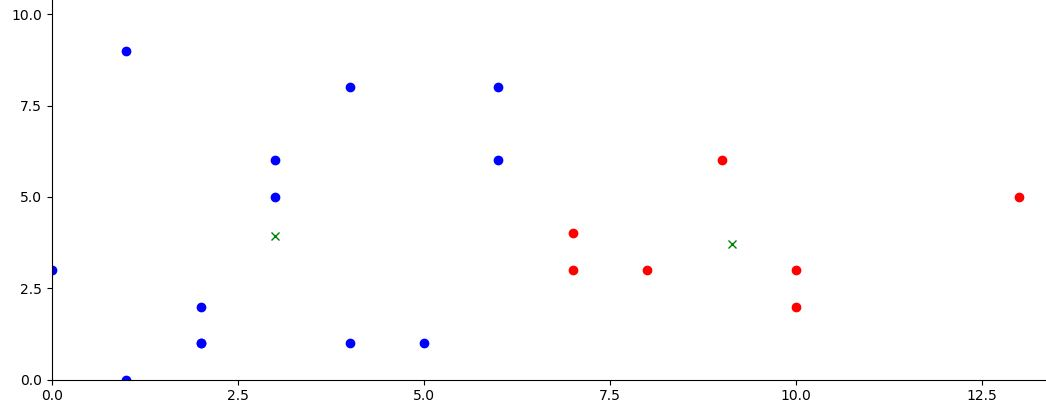
\includegraphics[scale=.5]{cluster_k2}
\caption{K = 2\newline Cluster Centers: \newline[9.142857142857142, 3.7142857142857144]\newline[3.0, 3.923076923076923]}
\label{fig:universe}
\end{figure}

\begin{figure}[h!]
\centering
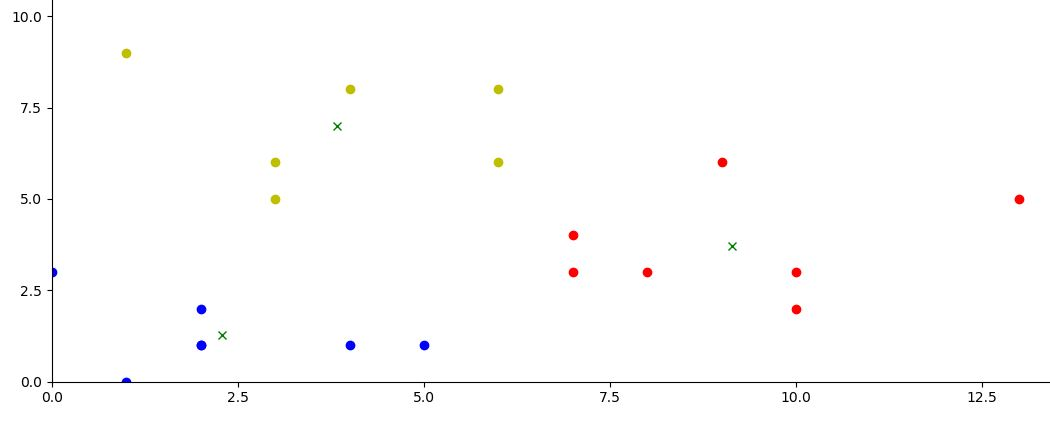
\includegraphics[scale=.5]{cluster_k3}
\caption{K = 3\newline Cluster Centers: \newline[9.142857142857142, 3.7142857142857144]\newline[2.2857142857142856, 1.2857142857142858]\newline[3.8333333333333335, 7.0]}
\end{figure}


\clearpage
\section {perceptron\_train(X,Y)}
This function takes the X values and the Y labels to recalculate the weight and bias for the samples. 
For the initial weights and bias there is a function that will initialize the weights to zero (set\_init(size)) and the bias is set to zero. Then for the number of samples, it will run a for loop that calculates the activation (get\_activation(X, weights, size, bias)). It will take that activation and multiply it by the label (check\_update(activation, Y)) and check if it is less then 0. If it is less then zero it needs to update. There is a function to update the weights (update\_weight(X, Y, weights, size)) and bias (update\_bias(bias, Y)) based on the previous values. If it is greater then 0 then it doesn't need to update. There is a variable that keeps track of how many updates there are and when it runs a full epoch without updates it will break out. If the number of non updates is not equal to the number of samples it will continue to run up to a preset value i chose which was a 100 epochs. When it gets to a hundred epochs it will break because we were not given a max epoch hyperparameter. When it is done it will put the weight and bias into list (append\_weights\_bias(weights, bias)) where W[0] are the weights and W[1] is the bias.

\section {perceptron\_test(X\_test, Y\_test, w, b)}
This function will take X\_test Y\_test and calculate the activation (get\_activation(X, weights, size, bias)) for each sample with the weights and bias that were passed in. It takes the activation and multiplies it by the label to check if it greater then zero (update\_bias(bias, Y)). If it is greater then zero that means it doesn't need to update and is correct. It will a variable that holds the number of correct and at the end return the number of correct over the number of samples. 

\section{Write-Up: Perceptron}
The weight for x1 is 2, weight for x2 is 4, and bias is 2. So this gives you the equation (2 * x1) + (4 * x2) + 2 = 0 which simplifies to x2 = -1/2 + (-1/2 * x1)

\begin{figure}[h!]
\centering
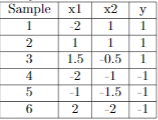
\includegraphics[scale=0.75]{perceptron_table.PNG}
\caption{Data the perceptron was built on}
\end{figure}


\begin{figure}[h!]
\centering
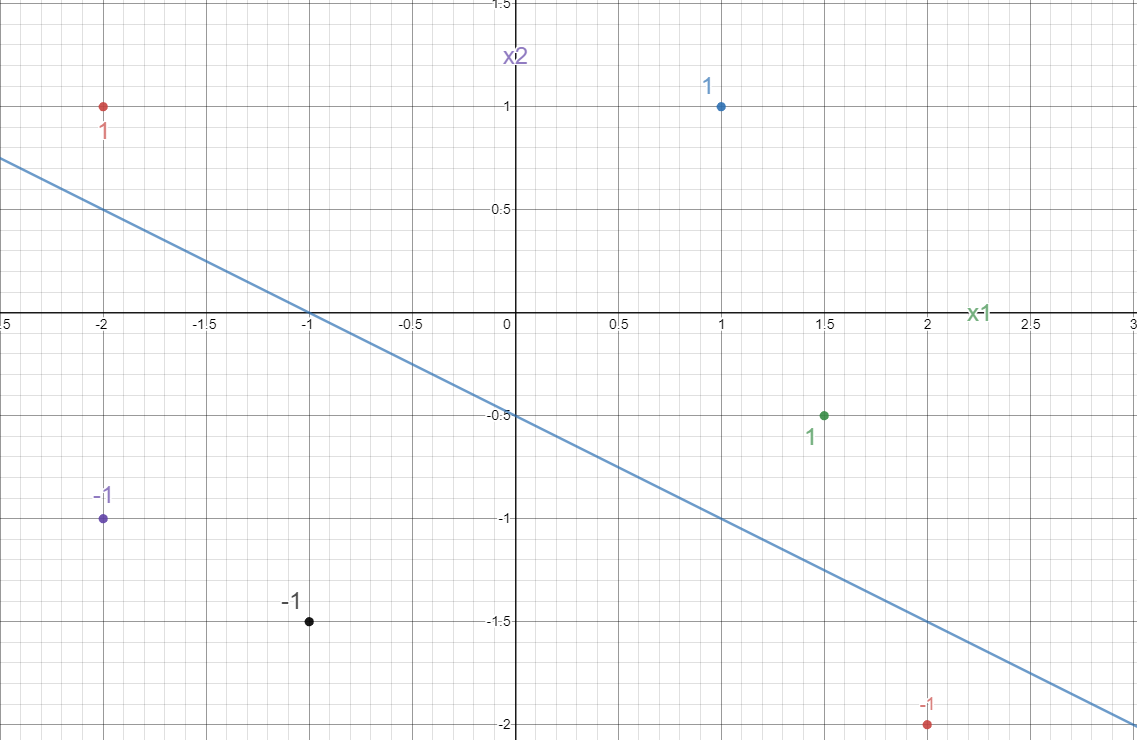
\includegraphics[scale=0.5]{perceptron.PNG}
\caption{Decision Boundary: x2 = -1/2 + (-1/2 * x1)\newline Also plots the samples in the datset}
\end{figure}

\end{document}

